\chapter{MNIST Multi-Layer Perceptron}

In this chapter we study the behavior of a simple multilayer perceptron (MLP) trained on the MNIST dataset. The objective is to understand how different hyperparameters affect training dynamics and model accuracy.



\section{Baseline Experiment}

We begin with a baseline configuration in order to observe the natural training dynamics of the MLP.

The network architecture is

\[
    784 \rightarrow 128 \rightarrow 10
\]

with ReLU activation and the Adam optimizer. The learning rate is $10^{-3}$ and the batch size is $64$.

During training we record the following quantities for each parameter tensor after every $25$ batches:
\begin{itemize}
    \item the $\ell_2$ norm of the gradient
    \item the $\ell_2$ norm of the parameters
    \item the ratio $\norm{\grad p} / \norm{p}$
\end{itemize}

These metrics (plotted in \cref{fig:mnist-mlp-exp01}) provide insight into the relative scale of updates during optimization.

\begin{figure}[tbp]
    \centering
    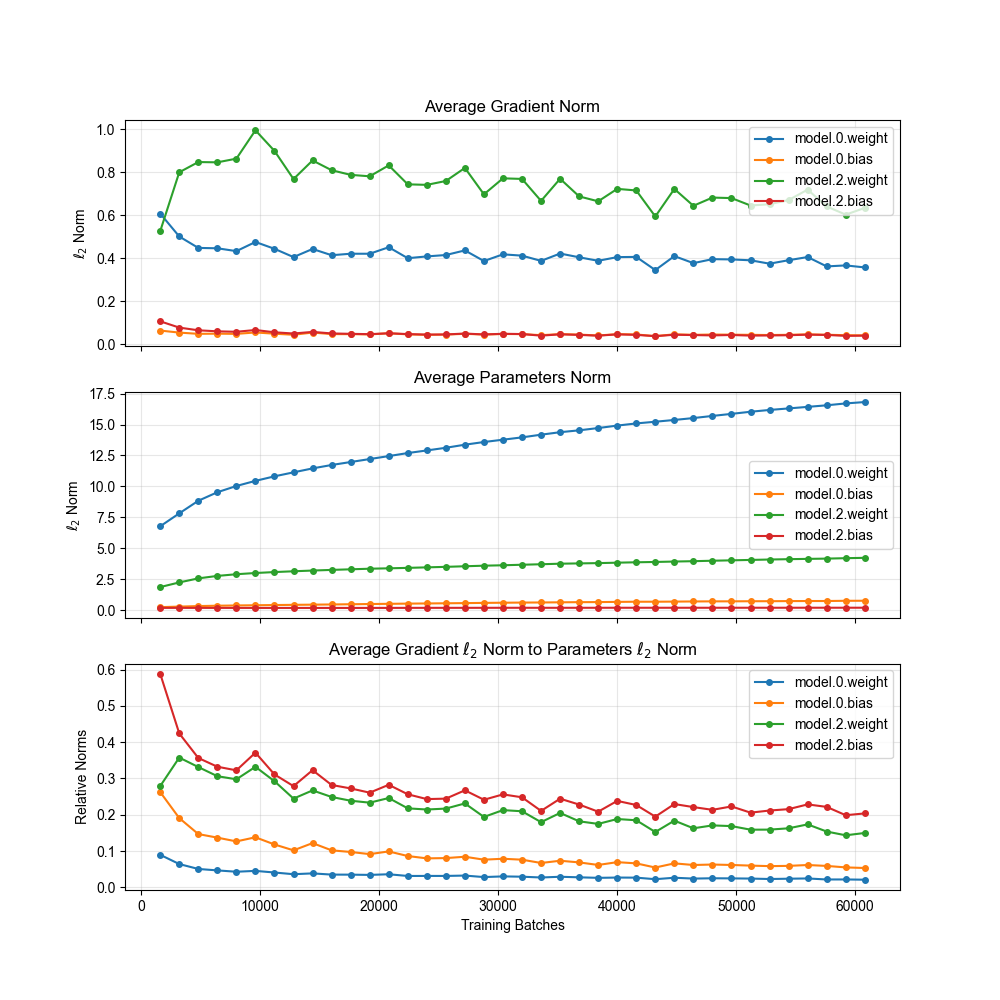
\includegraphics[width=\textwidth]{figures/mlp/exp01}
    \caption{Baseline metrics during training.}
    \label{fig:mnist-mlp-exp01}
\end{figure}

Several patterns can be observed:
\begin{enumerate}
    \item The gradient norms of the output layer are consistently larger than those of the first layer. This reflects the structure of backpropagation, where gradients are propagated through successive matrix multiplications and elementwise derivatives.

    \item The parameter norms increase steadily during training. This is expected because neural network weights are typically initialized with small magnitudes.

    \item The ratio $\norm{\grad p} / \norm{p}$ decreases over time. This indicates that parameter updates become relatively smaller as training progresses, suggesting convergence toward a stable region of the loss landscape.
\end{enumerate}




\section{Experiments}

Once a baseline is established, we can not study the effects of parameters such as the batch size and the learning rate on the MLP metrics. These experiments performed on the MLP with the values used for parameters are summarized in \cref{tab:mnist-mlp-exps}. The first row in this table shows the baseline experiment Exp~1.

\begin{table}[tbp]
    \centering

    \rowcolors{2}{tablegray}{white}

    \begin{eleganttable}{cccccc}
        \rowcolor{tableheader}
        \thead{Experiment} & \thead{Batch Size} & \thead{Learning Rate} & \thead{Epochs} & \thead{Accuracy (\%)} & \thead{Execution Time (s)} \\
        \midrule
        Exp 1  &  64   &  $10^{-3}$  &  1  &  94.13  &  10.469 \\
        Exp 2  &  128  &  $10^{-3}$  &  1  &  93.56  &  10.285 \\
        Exp 3  &  64   &  $10^{-4}$  &  1  &  89.69  &  10.294 \\
        Exp 4  &  64   &  $10^{-2}$  &  1  &  70.08  &  10.338 \\
    \end{eleganttable}

    \caption{Values used for MLP parameters in experiments to observe the metrics.}
    \label{tab:mnist-mlp-exps}
\end{table}


\subsection{Exp 2: Increasing the Batch Size}

Increasing the batch size reduces the variance of the gradient estimates, resulting in smoother gradient trajectories. However, the overall magnitude of the gradients and the evolution of parameter norms remain largely unchanged. This indicates that the batch size primarily influences stochastic noise rather than the expected optimization trajectory. When the noise is decreased as a result of the batch size, weights could land in a minima shaped like a sharp basin. Such minima are associated with poor generalization. That is why the accuracy slightly reduces. The computational efficiency is improved as we increase the batch size. This explains the reduction in the execution time. \cref{fig:mnist-mlp-exp02} shows the graphs of observed metrics.

\begin{figure}[tbp]
    \centering
    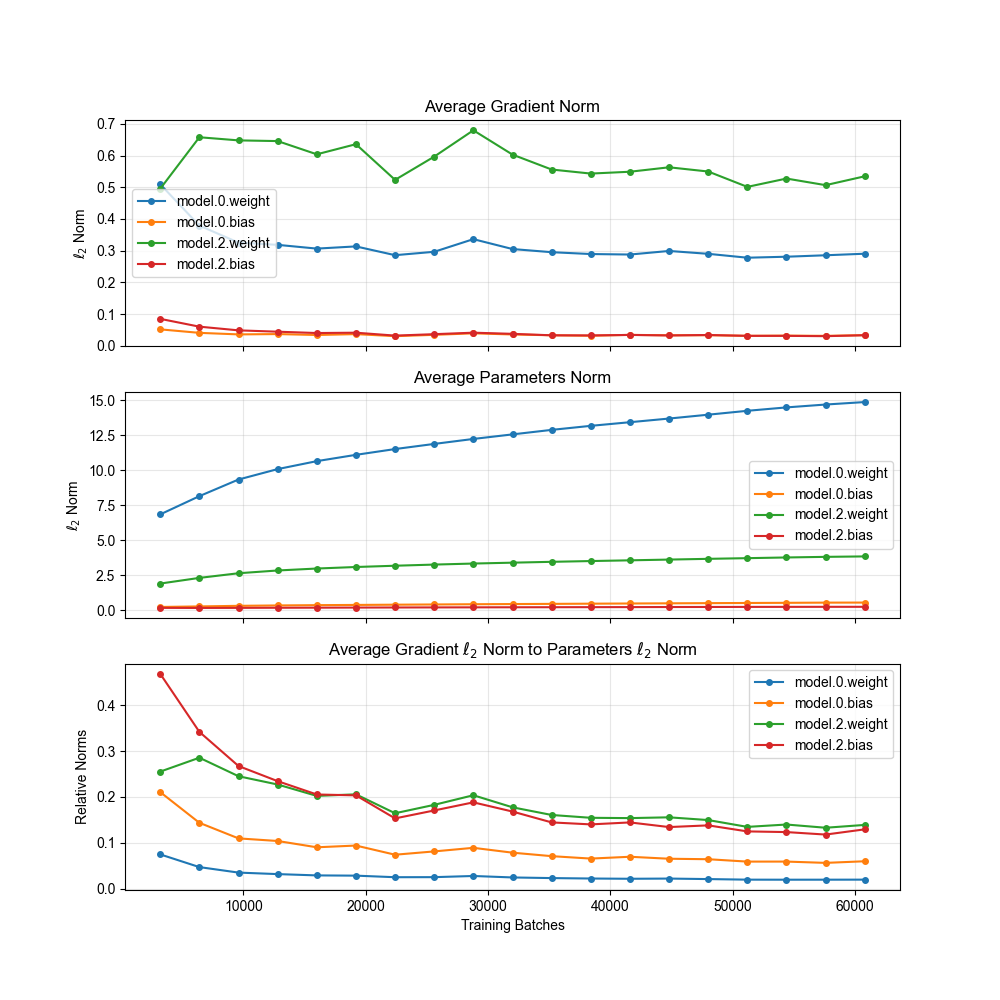
\includegraphics[width=\textwidth]{figures/mlp/exp02}
    \caption{Effects of increasing the batch size during training.}
    \label{fig:mnist-mlp-exp02}
\end{figure}


\subsection{Exp 3: Decreasing the Learning Rate}

Decreasing the learning rate reduces the step size taken during gradient descent. As a result, parameter updates become smaller and the parameters evolve more slowly during training. Consequently, the norms of the parameters increase at a slower rate compared to Exp~1, as shown in \cref{fig:mnist-mlp-exp03}.

Although the gradients themselves remain of comparable magnitude, the smaller learning rate reduces the effective update applied to the parameters at each step. This leads to slower progress toward a minimum of the loss function, which results in lower training effectiveness within a single epoch and therefore slightly reduced accuracy. The learning rate does not significantly affect the overall execution time since the same number of forward and backward passes are performed.

\begin{figure}[tbp]
    \centering
    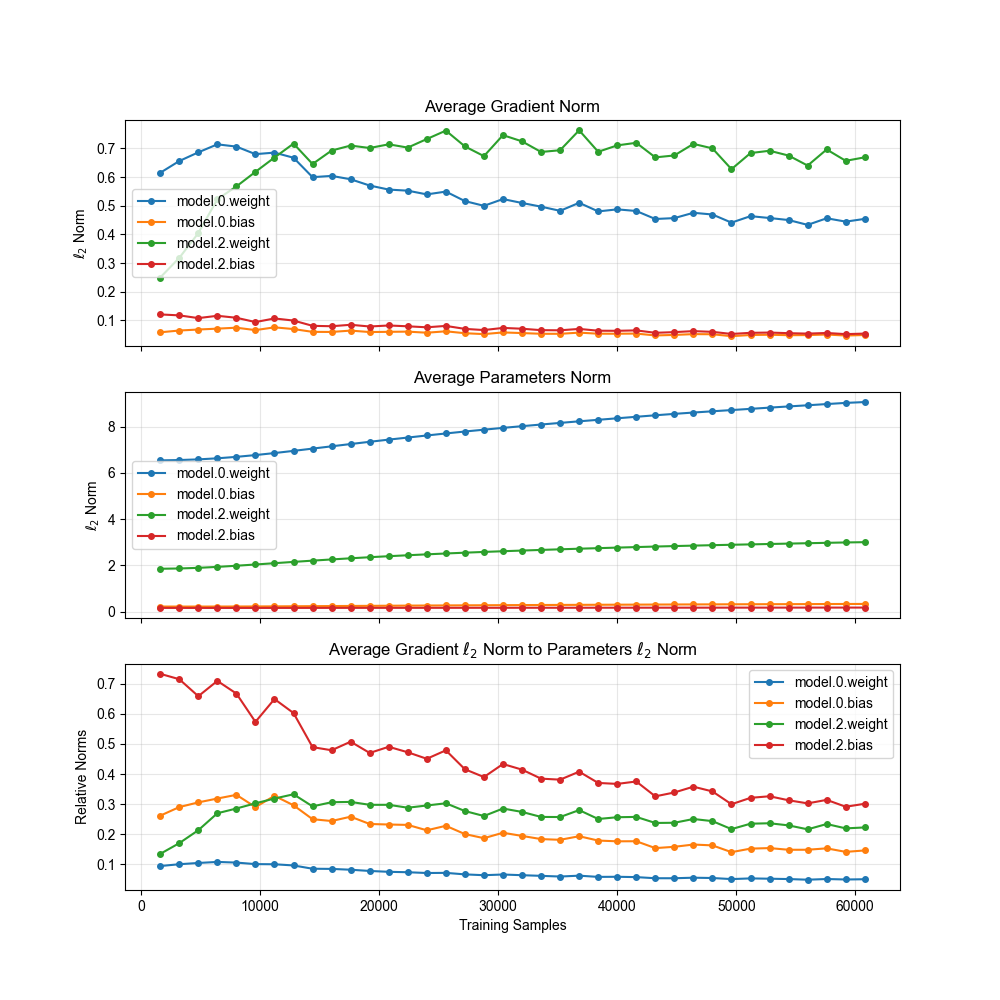
\includegraphics[width=\textwidth]{figures/mlp/exp03}
    \caption{Effects of decreasing the learning rate during training.}
    \label{fig:mnist-mlp-exp03}
\end{figure}


\subsection{Exp 4: Increasing the Learning Rate}

Increasing the learning rate further to $10^{-1}$ causes the optimizer to take very large steps during gradient descent. As a result, the parameters evolve too aggressively during training. This behavior is clearly visible in \cref{fig:mnist-mlp-exp04}, where the norms of the parameters grow extremely rapidly compared to previous experiments.

Although the gradient norms remain of comparable magnitude, the large learning rate amplifies the updates applied to the parameters at each iteration. These updates overshoot regions of lower loss in the loss landscape, preventing the optimizer from converging toward a stable minimum. Consequently, the training process becomes unstable and the final accuracy drops significantly to approximately $70\%$.

\begin{figure}[tbp]
    \centering
    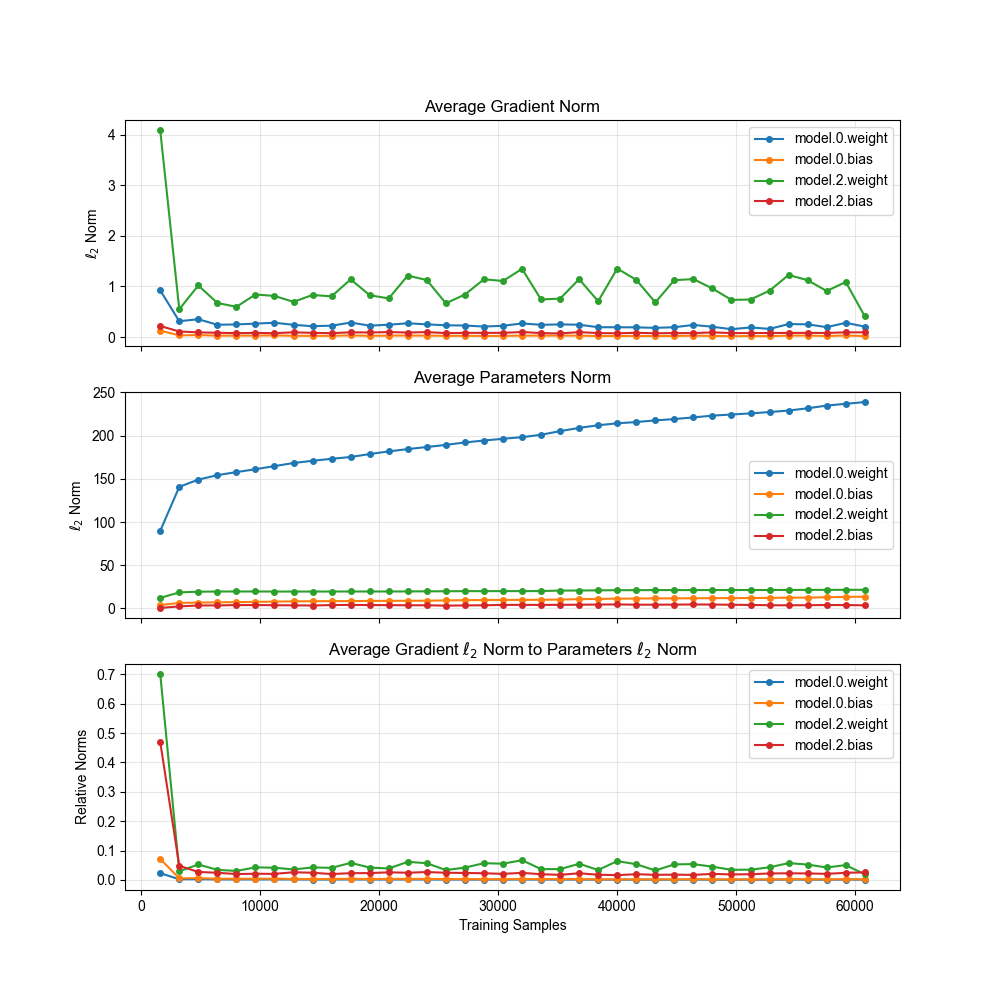
\includegraphics[width=\textwidth]{figures/mlp/exp04}
    \caption{Effects of increasing the learning rate during training.}
    \label{fig:mnist-mlp-exp04}
\end{figure}